\begin{refsection}

\chapter{U--Th--(Sm)--He}\label{ch:UThHe-R}

U--Th--(Sm)--He data are provided as flat tables with eight data
columns (Section~\ref{ch:UThHe}), in which the last two columns may be
empty if Sm has not been measured. They can be visualised on all the
generic plot devices, plus the helioplot. Before entering the U, Th,
Sm and He data into \texttt{IsoplotR}, they \textbf{must be corrected
  for \textalpha-ejection} using the procedures outlined in
Section~\ref{sec:alpha-ejection}.

\begin{center}
  \noindent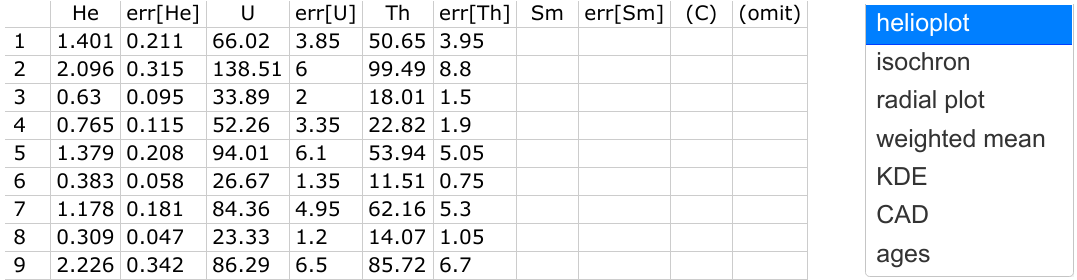
\includegraphics[width=.9\linewidth]{../figures/UThHeInputTablePlotDevices.png}
\end{center}

Note that, unlike all the other methods that were discussed before, it
is not necessary to specify the \texttt{format} argument when using
the \texttt{read.data()} function. \texttt{IsoplotR} automatically
figures out whether a dataset contains Sm or not:

\begin{script}
UThHe <- read.data('UThHe.csv',method='U-Th-He')
UThSmHe <- read.data('UThSmHe.csv',method='U-Th-He')
\end{script}

\noindent which returns a simple, eight-column table.\\

\noindent\begin{minipage}[t]{.65\linewidth}
\strut\vspace*{-\baselineskip}\newline
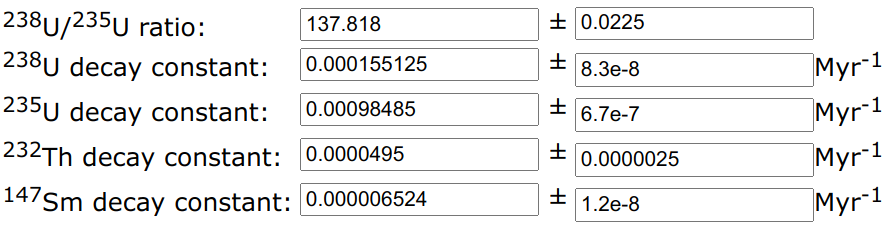
\includegraphics[width=\linewidth]{../figures/UThSmHeLambda.png}
\end{minipage}
\begin{minipage}[t]{.35\linewidth}
  The default U, Th and Sm decay constants are those of
  \citet{jaffey1971}, \citet{leroux1963} and \citet{villa2020}
  respectively.
\end{minipage}

\begin{script}
# change the Sm decay constant to the Lugmair and Marti (1978) value:
settings('lambda','Sm147',0.000006540,0.000000049)
\end{script}

\section{Helioplots}\label{sec:helioplot-R}

\texttt{IsoplotR}'s \texttt{helioplot} function represents a pair of
two plotting devices that visualise U--Th--He data as a compositional
data system (Section~\ref{sec:UThHeCompositional}).

\begin{enumerate}
  
\item \noindent\begin{minipage}[t]{.18\linewidth}
\strut\vspace*{-\baselineskip}\newline

\includegraphics[width=\linewidth]{../figures/UThHelioplotLogratio.png}
\end{minipage}
\begin{minipage}[t]{.82\linewidth}
  The compositional nature of the U--Th--He system can either be
  expressed as a logratio plot or a ternary diagram
  (Figure~\ref{fig:UThHeIsochronHelioplot}).\\
\end{minipage}

\begin{script}
oldpar <- par(mfrow=c(1,2)) # set up a two-panel plot
helioplot(UThHe,logratio=TRUE)  # logratio plot
helioplot(UThHe,logratio=FALSE) # ternary diagram
par(oldpar)
\end{script}

\item \noindent\begin{minipage}[t]{.28\linewidth}
\strut\vspace*{-\baselineskip}\newline

\includegraphics[width=\linewidth]{../figures/UThHeshownumbers.png}
\end{minipage}
\begin{minipage}[t]{.72\linewidth}
Tick the box to number the error ellipses by aliquot.\\
\end{minipage}

\begin{console}
helioplot(UThHe,show.numbers=TRUE)
\end{console}

\item\noindent\begin{minipage}[t]{.32\linewidth}
\strut\vspace*{-\baselineskip}\newline

\includegraphics[width=\linewidth]{../figures/UThHeCentralComposition.png}
\end{minipage}
\begin{minipage}[t]{.68\linewidth}
Ticking this box plots the geometric mean (`central') U--Th--He
composition and its covariance matrix as a white ellipse.
\end{minipage}

\begin{console}
helioplot(UThHe,show.central.comp=TRUE)
\end{console}

\item Overdispersion is treated similarly as in the context of
  regression (Section~\ref{sec:regression}) or the weighted mean
  (Section~\ref{sec:weightedmean}).

\noindent\begin{minipage}[t]{.45\linewidth}
\strut\vspace*{-\baselineskip}\newline
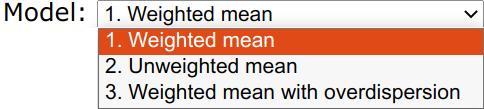
\includegraphics[width=\linewidth]{../figures/UThHeCentralAgeModels.png}
\end{minipage}
\begin{minipage}[t]{.55\linewidth}
Thus, there are options to augment the uncertainties with a factor
$\sqrt{\mbox{MSWD}}$ (model-1); to ignore the analytical uncertainties
altogether (model-2); or to add a constant overdispersion term to the
analytical uncertainties (model-3).
\end{minipage}

\begin{console}
helioplot(UThHe,model=1)
\end{console}

\item By default, the error ellipses and confidence intervals are
  shown at a 95\% confidence level ($\alpha=0.05$) and to
  2~significant digits.

\noindent\begin{minipage}[t]{.5\linewidth}
\strut\vspace*{-\baselineskip}\newline
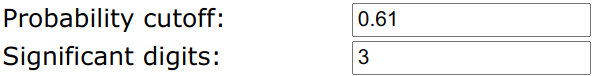
\includegraphics[width=\linewidth]{../figures/UThHealphasigdig.png}
\end{minipage}
\begin{minipage}[t]{.5\linewidth}
  Changing the significance level to $\alpha=0.61$ produces the
  equivalent of `1-sigma' confidence ellipses (and 39\% confidence
  intervals).
\end{minipage}

\begin{console}
helioplot(UThHe,alpha=0.61,sigdig=3)
\end{console}

\item The scaling settings of the \texttt{helioplot} function differ
  between the logratio and ternary option.

\noindent\begin{minipage}[t]{.5\linewidth}
\strut\vspace*{-\baselineskip}\newline
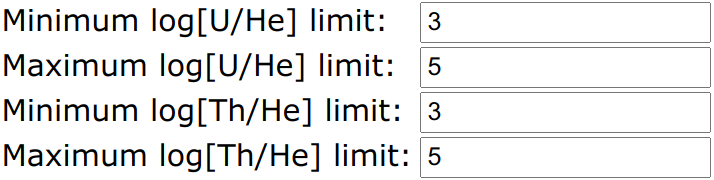
\includegraphics[width=\linewidth]{../figures/UThHeLogratioLimits.png}
\end{minipage}
\begin{minipage}[t]{.5\linewidth}
  The horizontal and vertical extent of the logratio plot is
  controlled by the log(U/He) and log(Th/He) limits (where `log'
  stands for the natural logarithm).
\end{minipage}

\begin{console}
helioplot(UThHe,logratio=TRUE,xlim=c(3,5),ylim=c(3,5))
\end{console}

For the ternary diagram, scaling is achieved via a three-element
vector of multipliers for He, Th and U, respectively.  The default
scaling automatically selects scaling factors that place the geometric
mean composition of the data at the barycentre of the ternary diagram.

\noindent\begin{minipage}[t]{.4\linewidth}
\strut\vspace*{-\baselineskip}\newline
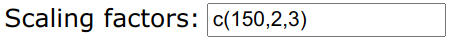
\includegraphics[width=\linewidth]{../figures/UThHeFact.png}
\end{minipage}
\begin{minipage}[t]{.6\linewidth}
Entering \texttt{c(150,2,3)} multiplies the He abundance with 150, the
Th abundance with 2 and the U abundance with 3 before re-normalising
and plotting on the ternary diagram.
\end{minipage}

\begin{console}
helioplot(UThHe,logratio=FALSE,fact=c(150,2,3))
\end{console}

\item\noindent\begin{minipage}[t]{.5\linewidth}
\strut\vspace*{-\baselineskip}\newline
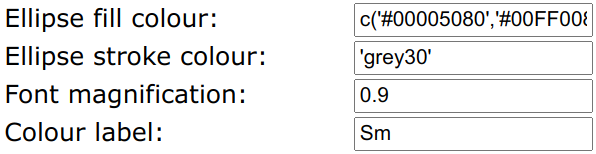
\includegraphics[width=\linewidth]{../figures/UThHeEllipseColours.png}
\end{minipage}
\begin{minipage}[t]{.5\linewidth}
  The fill and stroke colours of the error ellipses can be used to
  represent additional information such as the Sm-concentration of the
  various aliquots.
\end{minipage}

\begin{script}
helioplot(UThSmHe,levels=UThSmHe[,'Sm'],clabel='Sm',
          ellipse.fill=c('#00005080','#00FF0080'),
          ellipse.stroke='grey30')
\end{script}

\end{enumerate}

\section{Ages and other plots}

\begin{enumerate}
  
\item \texttt{IsoplotR}'s \texttt{isochron()} function uses the linear
  age approximation (Equation~\ref{eq:t=HeP}) to create a
  \textit{pseudo-isochron} through multiple aliquots of the same
  sample.  Recall that this approximation sets out the helium
  concentration against the present-day \textalpha-production rate,
  which is a function of the U, Th and Sm concentrations.

Because U, Th and Sm are measured separately from He (and on a
different mass spectrometer), the analytical uncertainties of the two
isochron variables can safely be assumed to be zero. Therefore, a
U--Th--He isochron consists of error crosses rather than error
ellipses.  Apart from this small difference, all the other parameters
are the same as for generic regression function
(Section~\ref{sec:OtherRegression}) and isochron plots that were
previously discussed.

\begin{console}
isochron(UThHe)
\end{console}

\item Calculating single grain ages is easier for the U--Th--He method than
it is for any other method discussed so far. This is because the
inherited daughted component can be neglected, given the low abundance
of helium in the atmosphere, and its low solubility in minerals and
melts. Therefore, \texttt{IsoplotR}'s \texttt{age()} function has very
few options.

\begin{console}
age(UThHe)
\end{console}

\item\noindent\begin{minipage}[t]{.5\linewidth}
\strut\vspace*{-\baselineskip}\newline
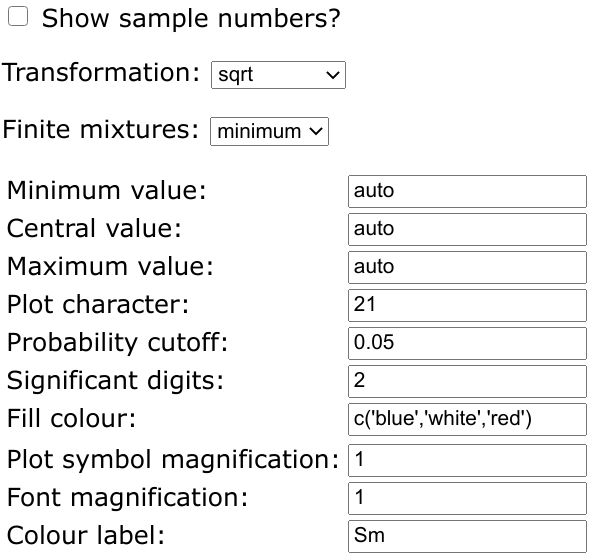
\includegraphics[width=\linewidth]{../figures/UThHeRadial.png}
\end{minipage}
\begin{minipage}[t]{.5\linewidth}
The resulting single grain ages can be visualised on radial, weighted
mean, KDE and CAD plots. These work in exactly the same way as the
generic \texttt{radialplot()} (Section~\ref{sec:OtherRadial}),
\texttt{weightedmean()} (Section~\ref{sec:OtherWeightedMean}),
\texttt{kde()} (Section~\ref{sec:OtherKDE}) and \texttt{cad()}
(Section~\ref{sec:OtherCAD}) functions. For example, this screenshot
shows a radial plot using a square root transformation, with grains
coloured by Sm-content, using a three-colour scale, and applying the
minimum age model of Section~\ref{sec:mixtures}. All other settings
use the default values.
\end{minipage}
  
\begin{script}
radialplot(UThSmHe,transformation='sqrt',k='min',clabel='Sm',
           levels=UThSmHe[,'Sm'],bg=c('blue','white','red'))
\end{script}

Plotting the same data on a weighted mean diagram, using the random
effects model and ranking the aliquots by age:

\begin{script}
weightedmean(UThSmHe,random.effects=TRUE,ranked=TRUE,clabel='Sm',
             levels=UThSmHe[,'Sm'],rect.col=c('blue','white','red'))
\end{script}

Plotting \texttt{UThSmHe} as a KDE from 5 to 12~Ma, and using a log
scale because of the high coefficient of variation:

\begin{console}
kde(UThSmHe,log=TRUE,from=5,to=12)
\end{console}

Showing the same data as a CAD (which uses a linear scale):

\begin{console}
cad(UThSmHe)
\end{console}

\end{enumerate}

\printbibliography[heading=subbibliography]

\end{refsection}
